\section{Evaluation\label{evaluation}}

\begin{figure}
  \centering
      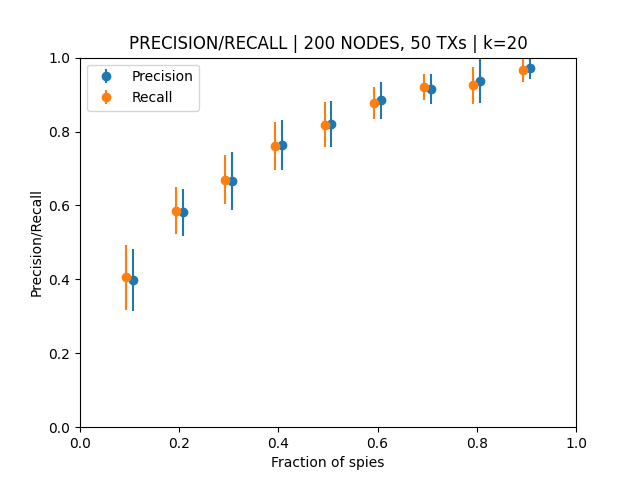
\includegraphics[width=0.5\textwidth]{figs/nodand}
  \caption{First Spy Estimator Kadcast}
  \label{fig:nodand}
\end{figure}

\begin{figure}
  \centering
      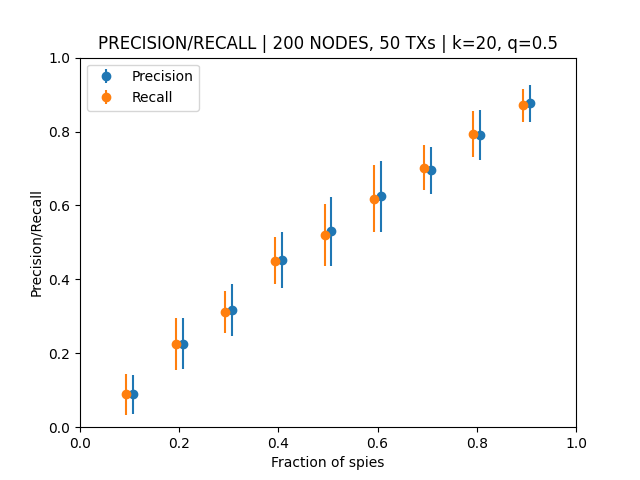
\includegraphics[width=0.5\textwidth]{figs/dand05}
  \caption{First Spy Estimator Kadcast with Dandelion}
  \label{fig:dand}
\end{figure}

To evaluate the privacy properties of Kadcast we ran multiple simulations of
transaction broadcasting with the Kadcast algorithm. Each simulation has
the same amount of overall active nodes in the network (200) and overall
sent transactions (50). [TODO begründung für die werte/experimente
nochmal mit begründeteren werten laufen lassen]
We ran each simulation for different fractions of spies.
The transactions are sent only by benign nodes, and all transactions are
randomly distributed among the benign nodes. Not each node does have to
send a transaction and some nodes may send multiple transactions.
For each network configuration we created 20 samples and averaged the
results. We show the means and standard deviations in each plot. \\
In our first experiment, we take a look at how the first spy estimator would perform in a standard setting,
using Kadcast with parameters used in real world scenarios, i.e. an
ID length of 160 bits and a bucket size of 20.
Messages are distributed by first sending the broadcast to the
largest subtree, and then iteratively sending it to the other subtrees in
descending order. \\
The results of the ``standard settings'' simulation can be seen in
Figure~\ref{fig:nodand}. \\
%The figure includes averaged precision and recall values and the standard deviation of our measurements. \\
We see that the first spy estimator performs relatively well.
Even with an amount of as low as 20\% of spies, the attacker can
map over half of the sent transactions correctly.
These results further reinforce our working hypothesis. \\
We wanted to test if the bucket size has any
meaningful correlation to the performance of the estimator. We therefore
repeated our experiment with common bucket sizes, the results can be
seen in Figure~\ref{fig:allk_r} [In meiner
Vorstellung waren die Plots schöner].
Different $k$ values did not have an effect on the anonymity
properties in our network configuration. \\
We further wanted to know if we can improve the anonymity by using
Dandelion spreading[fanti].
Therefore we implemented a simple version of the Dandelion algorithm. It
uses the $q$ parameter as described in the original dandelion
paper[dand1],
to decide at each hop if the algorithm should stop the anonymity phase
and start the broadcasting phase. The $q$ value is the probability to leave
the anonymity phase at each hop. We did not build a Hamiltonian circuit as
described by [fanti et. al], but just used a random (loopfree) path through
the graph for each transaction. Therefore our approach is a simplified
version of Dandelion, similar to a more traditional
``diffusion-by-proxy'' [] approach. Nevertheless, this addition has some observable
positive effects on the anonymity of our network. The results of 
combining Kadcast with this simplified Dandelion spreading, using
the standard parameter $q = 0.5$, can be seen in \ref{fig:dand}. Compared to
standard Kadcast this is a massive improvement. Using Dandelion, the
estimator performs worse in every network configuration, for every
amount of spies. \\
We can also observe that the effectiveness of
the estimator scales linearly to the fraction of spies when using Dandelion, while it
increases logarithmically when using Kadcast without Dandelion [TODO was
sagt uns das?]. \\
We ran the experiment again for different $q$ values, the results can
be seen in Figure~\ref{fig:allq_r}.

\begin{figure}
  \centering
      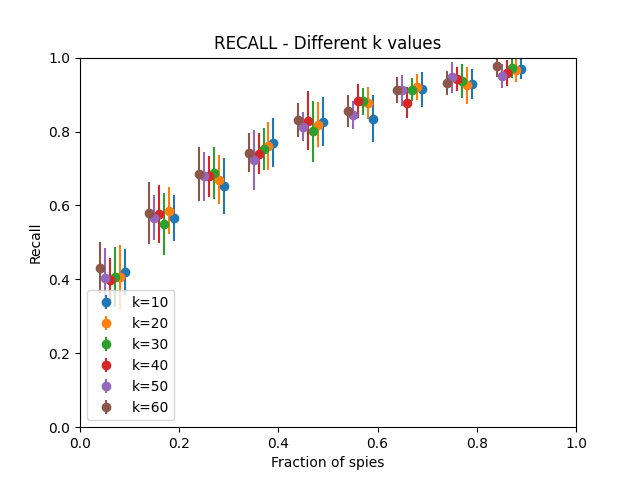
\includegraphics[width=0.5\textwidth]{figs/allks_recall}
  \caption{Recall values for different bucket sizes}
  \label{fig:allk_r}
\end{figure}

%\begin{figure}
%  \centering
%      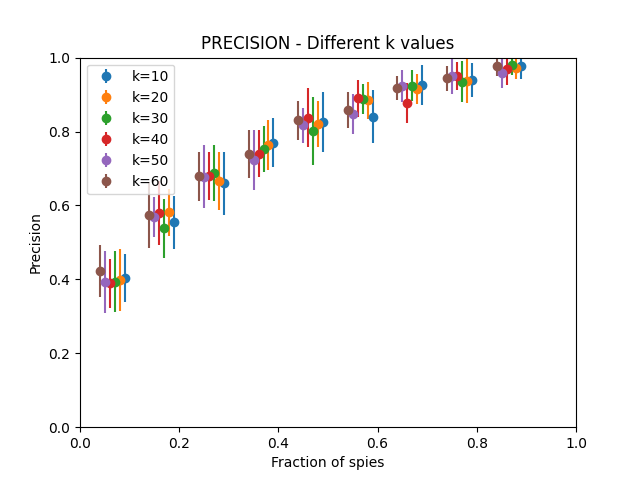
\includegraphics[width=0.5\textwidth]{figs/allks_precision}
%  \caption{Precision values for different bucket sizes}
%  \label{fig:allk_p}
%\end{figure}

\begin{figure}
  \centering
      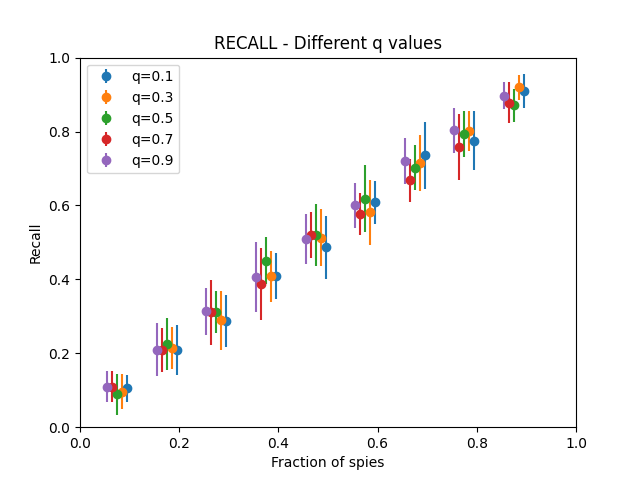
\includegraphics[width=0.5\textwidth]{figs/allqs_recall}
  \caption{Recall values for different Dandelion q values}
  \label{fig:allq_r}
\end{figure}

[TODO erklären warum hier auf einmal nur noch recall und nicht mehr
precision ist]
The results indicate that it does not make a
difference if the anonymity phase is long or short. Instead, we see a
similar net increase in anonymity for all $q$ values. \\
As Dandelion only adds a constant overhead to the overall broadcast time [source
dand1fanti], we think it would be a meaningful addition to Kadcast,
especially if we take the bad results we have observed in our standard
Kadcast experiments into consideration.
